% This file was adapted from ICLR2022_conference.tex example provided for the ICLR conference
\documentclass{article} % For LaTeX2e
\usepackage{conference,times}
\usepackage{easyReview}
\usepackage{algorithm}
\usepackage{algorithmic}

% Optional math commands from https://github.com/goodfeli/dlbook_notation.
\input{math_commands.tex}

\usepackage{amsthm,amssymb}

\newtheorem{theorem}{Theorem}[section]
\newtheorem{corollary}{Corollary}[theorem]
\newtheorem{lemma}[theorem]{Lemma}
\newtheorem{definition}[theorem]{Definition}

% Please leave these options as they are
\usepackage{hyperref}
\hypersetup{
    colorlinks=true,
    linkcolor=red,
    filecolor=magenta,
    urlcolor=blue,
    citecolor=purple,
    pdftitle={Detecting Physical and Procedural Bias in Lottery Draws: A Number-Theoretic and Statistical Study},
    pdfpagemode=FullScreen,
    }



\title{Detecting Physical and Procedural Bias in Lottery Draws: \\
A Number-Theoretic and Statistical Study}

\author{Marius-Constantin Dinu \\
Independent Researcher \\
\texttt{marius.constantin.dinu@example.com}}

\begin{document}


\maketitle

\begin{abstract}
Physical lottery systems are designed to approximate uniform sampling without replacement, yet practical implementations involve latent mechanical and procedural factors that can induce weak, time-varying departures from ideal randomness. This paper develops a hybrid inferential and predictive framework that integrates regime diagnostics, dependence-aware multiplicity control, bounded-confounding identification, staged transfer evaluation, and reliability-constrained integrated scoring. The objective is explicitly non-deterministic: we test reproducible structure and uncertainty bounds rather than deterministic prediction of winning combinations. We formalize five optimization/identification programs with explicit decision variables, feasible sets, and optimality criteria, and we provide complete theorem and lemma proofs for the key guarantees used by the pipeline. On a long-horizon historical draw corpus, evidence is asymmetric: confounding-robust directional interpretation and strict false-discovery control are strong, while segmentation stability and integrated score dominance remain below pre-registered gates. The resulting contribution is methodological and practical: robust bias-screening claims can be made with high transparency under severe observability limits, while integrated-superiority claims should remain conditional until targeted reruns resolve the remaining gates.
\end{abstract}

\section{Introduction}
Lottery fairness is mathematically simple under ideal assumptions and empirically difficult under real operation. In theory, draws follow exact combinatorial laws induced by game rules; in practice, draws are generated by physical machines, evolving ball sets, procedural handling, and rule-era transitions that may introduce weak structure. The inferential challenge is therefore not only to test a global null, but to isolate persistent and reproducible departures from random fluctuation while controlling multiplicity and temporal instability.

This challenge has cross-domain significance. Similar conditions appear in manufacturing quality surveillance, regulatory anomaly monitoring, and other stochastic audit settings where latent mechanisms are only partially observed. In these settings, overclaiming can be more harmful than underclaiming, so methodological discipline requires explicit tests of stationarity, dependence, confounding sensitivity, and holdout replication before strong conclusions are issued \citep{S20,S21,S24,S32,S33}.

Classical time-series and multiple-testing literatures provide strong ingredients but not a unified pipeline. Unit-root and stationarity tools diagnose pooled-assumption validity \citep{S01,S02,S03,S04}. Linear and nonlinear dependence diagnostics expose residual structure \citep{S05,S06,S07}. Structural-break methods detect regime transitions in long sequences \citep{S08,S09,S10,S11,S12,S13,S14,S27,S28,S37}. False-discovery frameworks and empirical-null corrections calibrate large feature scans under dependence \citep{S15,S16,S17,S18,S19,S25,S26}. Randomness battery literature warns that multi-test screening is informative but not equivalent to mechanism identification \citep{S20,S21,S22,S23,S24,S38}. Domain studies and official operator sources provide valuable context but still leave substantial observability gaps \citep{S29,S30,S34,S35,S36,S39}.

This paper integrates these ingredients into a staged architecture anchored to explicit gate logic. Regime segmentation is estimated first, discovery is constrained by both false-discovery and temporal replication criteria, directional interpretation is filtered by bounded-confounding intervals, transfer modeling is evaluated through staged non-inferiority and optional superiority checks, and final integrated ranking is recalibrated by a reliability-constrained max-min objective. Every major claim is tied to a concrete figure or table.

The main contributions are:
\begin{itemize}
\item We define a calibrated segmentation program with finite-feasible optimality guarantees and explicit penalties for diagnostic inconsistency, linking boundary selection to inferential reliability.
\item We formalize prefix-optimal discovery under dependence-aware false-discovery control and replication constraints, with a complete optimality proof for the nested family.
\item We derive an exact sign-identification boundary under bounded latent confounding, turning mechanism-direction claims into testable inequalities.
\item We introduce a staged transfer protocol with mandatory non-inferiority and optional superiority, and we prove gate-safety logic that blocks invalid superiority claims.
\item We formulate reliability-constrained max-min score recalibration and prove a conic impossibility condition for universal fixed-weight dominance across baselines.
\end{itemize}

The paper structure is as follows. \Secref{sec:related} contrasts related methods and identifies the unresolved gap. \Secref{sec:problem} defines symbols, assumptions, and optimization objects. \Secref{sec:method} presents architecture, pseudocode, and core proofs. \Secref{sec:protocol} details evaluation and reproducibility settings. \Secref{sec:results} provides evidence-linked findings. \Secref{sec:limitations} states current boundary conditions and future experiments needed to improve claim strength. \Secref{sec:conclusion} summarizes implications.

\section{Related Work}\label{sec:related}
\subsection{Diagnostics and Structural Change}
Stationarity and dependence diagnostics are fundamental for deciding whether pooled inference is valid. Unit-root and stationarity frameworks \citep{S01,S02,S03,S04} and residual-dependence tests \citep{S05,S06,S07} make assumptions auditable rather than implicit. Their strength is interpretability; their limitation is that they do not by themselves choose changepoints.

Structural-break and changepoint methods address that limitation \citep{S10,S11,S12,S13,S14,S27,S28,S37}. Exact and near-linear algorithms make long historical sequences tractable, but practical outputs can be penalty-sensitive and often disconnected from downstream multiplicity behavior. Our approach retains these tools while embedding diagnostic penalties directly in the segmentation objective so boundary quality is coupled to inferential objectives rather than treated as an isolated preprocessing choice.

\subsection{Multiplicity, Replication, and Empirical Nulls}
BH/BY procedures remain central for false-discovery control under broad dependence assumptions \citep{S15,S16}. Q-value and empirical-null approaches improve calibration-power balance in large-scale testing \citep{S17,S18,S19}. Newer robust procedures extend these ideas to generalized and nonstandard settings \citep{S25,S26}. The unresolved issue in longitudinal audits is that single-era significance is often unstable across time.

We address this by directly constraining discovery with temporal replication, not only adjusted p-values. In effect, a descriptor must satisfy inferential control and out-of-period persistence jointly. This shifts the optimization target from maximal rejection count to maximal reproducible discovery.

\subsection{Randomness Testing and Domain Context}
Randomness battery literature provides a key caution: passing or failing batteries is screening evidence, not direct mechanism attribution \citep{S20,S21,S24,S38}. Lottery-focused studies \citep{S29,S30} and governance sources \citep{S32,S33,S34,S35,S36} provide operational context but typically do not integrate regime uncertainty, confounding bounds, and transfer evaluation in one end-to-end protocol.

The gap motivating this manuscript is therefore hybrid. Prior work offers strong components but not a single assumption-consistent chain from regime identification through reproducibility-constrained inference and reliability-aware integrated ranking under explicit gate logic.

\section{Problem Setting and Formal Definitions}\label{sec:problem}
\subsection{Data, Spaces, and Standing Assumptions}
Let draws be indexed by $t=1,\ldots,T$, with observed outcome vector $x_t\in\Omega_{r(t)}$, where $\Omega_r$ is the rule-era sample space and $r(t)$ is an unknown regime map. A descriptor map $\phi$ yields $z_t=\phi(x_t)\in\mathbb{R}^p$. Temporal partitions are denoted by $\train$, $\valid$, and $\test$, and threshold tuning is restricted to pre-registered source/validation windows.

The method uses five standing assumptions. (A1) Candidate changepoints lie on a finite grid with minimum spacing. (A2) Null probabilities are computed on regime-consistent combinatorial spaces. (A3) Holdout windows are never used for exploratory threshold tuning. (A4) Latent mechanism covariates are unobserved but can be bounded in sensitivity form. (A5) Integrated scoring must satisfy reliability floors before competitiveness claims are interpreted.

\subsection{Calibrated Regime Segmentation}
Define changepoints $\tau=(\tau_1,\ldots,\tau_M)$ with feasibility set
\[
\mathcal{T}_{L_{\min}}=\{\tau:0=\tau_0<\tau_1<\cdots<\tau_M<\tau_{M+1}=T,\;\tau_{m+1}-\tau_m\ge L_{\min}\}.
\]
Let $\mathcal{C}^{\star}_m(\tau)$ be profiled segment cost, $A_m(\tau)\in\{0,1\}$ a diagnostic alarm indicator, and $N_{\mathrm{IID}}(\tau)$ the expected false-boundary count under an era-faithful IID surrogate. The calibrated objective is
\begin{equation}
\hat{\tau}\in\arg\min_{\tau\in\mathcal{T}_{L_{\min}}}
J_{\mathrm{seg}}(\tau)
=\sum_{m=0}^{M}\mathcal{C}^{\star}_m(\tau)+\beta M+\lambda\sum_{m=0}^{M}A_m(\tau)+\kappa N_{\mathrm{IID}}(\tau).
\label{eq:segmentation}
\end{equation}
Decision variable: $\tau$. Feasible set: $\mathcal{T}_{L_{\min}}$. Optimality criterion: global minimum of $J_{\mathrm{seg}}$.

\subsection{Replication-Constrained Prefix Discovery}
Descriptors are ranked to induce nested prefixes $\mathcal{R}_k$. Let $F_k$ denote dependence-aware false-discovery estimate and $\rho_k$ the holdout replication fraction.
\begin{equation}
\hat{k}=\arg\max_{0\le k\le p}k
\quad\text{s.t.}\quad F_k\le q,\;\rho_k\ge\rho_0.
\label{eq:prefix}
\end{equation}
Decision variable: $k$. Feasible set: indices satisfying both constraints. Optimality criterion: maximal feasible prefix size.

\subsection{Bounded-Confounding Sign Identification}
For descriptor $j$ in regime $r$, write
\begin{equation}
\Delta_{jr}=b_{jr}+\gamma_j u_r,\qquad |u_r|\le\Gamma,
\label{eq:confounding-model}
\end{equation}
with implied interval
\begin{equation}
\mathcal{I}_{jr}(\Gamma)=\big[\Delta_{jr}-|\gamma_j|\Gamma,\;\Delta_{jr}+|\gamma_j|\Gamma\big].
\label{eq:confounding}
\end{equation}
Decision variable: sign-identifiable versus ambiguous classification. Feasible set: bounded-confounding class indexed by $\Gamma$. Optimality criterion: valid directional claims only when zero is excluded from \eqref{eq:confounding}.

\subsection{Staged Stability-Regularized Transfer}
For auxiliary target $y_t$, feature vector $g_t$, regime indices $\mathcal{I}_r$, and coefficients $\beta_r\in\mathbb{R}^d$, solve
\begin{equation}
\hat{\beta}_{1:R}\in\arg\min_{\beta_{1:R}}
\sum_{r=1}^{R}\sum_{t\in\mathcal{I}_r}\ell\big(y_t,\sigma(\beta_r^\top g_t)\big)
+\eta\sum_{r=2}^{R}\|\beta_r-\beta_{r-1}\|_1
+\lambda\sum_{r=1}^{R}\|\beta_r\|_1.
\label{eq:fused}
\end{equation}
Decision variables: $\beta_{1:R}$. Feasible set: all coefficient vectors on fixed admissible features. Optimality criterion: global convex minimizer.

Stage-A gate (mandatory) requires non-inferiority in transport calibration; Stage-B gate (optional) allows superiority claims only if Stage-A passes first.

\subsection{Reliability-Constrained Max-Min Score Recalibration}
Let $m(P)\in[0,1]^K$ be normalized metric vector for pipeline $P$, baseline set $\mathcal{B}$, and simplex $\Delta^K=\{w\ge0,\sum_k w_k=1\}$. Denote the integrated pipeline by $P_{\mathrm{int}}$. Reliability floors are $m_{\mathrm{FDR}}(P_{\mathrm{int}})\ge c_1$ and $m_{\mathrm{sign}}(P_{\mathrm{int}})\ge c_2$. The weight optimization is
\begin{equation}
\hat{w}\in\arg\max_{w\in\Delta^K}\;\min_{b\in\mathcal{B}}\left[w^\top m(P_{\mathrm{int}})-w^\top m(b)\right]
\quad\text{s.t.}\quad m_{\mathrm{FDR}}(P_{\mathrm{int}})\ge c_1,\;m_{\mathrm{sign}}(P_{\mathrm{int}})\ge c_2.
\label{eq:maxmin}
\end{equation}
Decision variable: $w$. Feasible set: simplex plus reliability constraints. Optimality criterion: maximize worst-case baseline margin under inferential floors.

\section{Integrated Methodology}\label{sec:method}
\subsection{Architecture and Module Responsibilities}
The method is implemented as a five-module architecture aligned with \eqref{eq:segmentation}, \eqref{eq:prefix}, \eqref{eq:confounding}, \eqref{eq:fused}, and \eqref{eq:maxmin}. Module 1 estimates regime partitions with diagnostic and IID-null calibration. Module 2 performs multiplicity-controlled prefix discovery with replication constraints. Module 3 applies bounded-confounding sign identification. Module 4 trains and evaluates staged transfer models with explicit gate logic. Module 5 recalibrates integrated scoring through reliability-constrained max-min weighting.

This decomposition localizes failure modes and prevents leakage. Weak segmentation consensus cannot be hidden by discovery metrics; transfer gains cannot bypass inferential floors; and integrated rankings cannot be interpreted without reliability checks. The architecture is therefore designed for claim calibration, not merely score maximization.

\subsection{Workflow Pseudocode}
\begin{algorithm}[t]
\caption{Integrated bias-detection and reliability-calibrated ranking workflow}
\label{alg:pipeline}
\begin{algorithmic}
\STATE Input draws $\{x_t\}_{t=1}^T$, descriptor map $\phi$, seed set $\mathcal{S}$, and sweep grids
\STATE Build descriptors $z_t=\phi(x_t)$ and candidate boundary grid
\STATE Solve \eqref{eq:segmentation}; freeze regime partition and diagnostics
\STATE Compute descriptor p-values and holdout replication indicators
\STATE Solve \eqref{eq:prefix} to obtain reproducible descriptor subset
\STATE For each retained descriptor, evaluate interval logic in \eqref{eq:confounding}
\STATE Keep sign-identifiable effects and construct transfer features
\STATE Fit staged transfer model via \eqref{eq:fused}; evaluate Stage-A and Stage-B gates
\STATE Solve reliability-constrained score recalibration in \eqref{eq:maxmin}
\STATE Run conic-impossibility diagnostic and report uncertainty-aware evidence tables
\end{algorithmic}
\end{algorithm}

\Algref{alg:pipeline} imposes strict dependency ordering: downstream claims are valid only if upstream assumptions and gates remain satisfied.

\subsection{Core Formal Guarantees}
\begin{theorem}[Existence of calibrated segmentation minimizer]
Assume candidate boundaries form a finite feasible set under spacing constraints and each term in \eqref{eq:segmentation} is finite for feasible $\tau$. Then the argmin of \eqref{eq:segmentation} is non-empty.
\label{thm:segexist}
\end{theorem}
\begin{proof}
By finite-grid and spacing assumptions, $\mathcal{T}_{L_{\min}}$ is finite. The objective in \eqref{eq:segmentation} maps each feasible $\tau$ to a real number because all terms are finite by assumption. Any real-valued function on a finite set attains a minimum, so at least one global minimizer exists. \qedhere
\end{proof}

\begin{lemma}[Largest feasible prefix is optimal]
Let $\mathcal{K}=\{k:F_k\le q,\rho_k\ge\rho_0\}$ from \eqref{eq:prefix} be non-empty. If $k^{\star}=\max\mathcal{K}$, then $k^{\star}$ solves \eqref{eq:prefix}.
\label{lem:prefix}
\end{lemma}
\begin{proof}
Every feasible solution corresponds to one $k\in\mathcal{K}$ with objective value $k$. Since $k^{\star}$ is maximal in $\mathcal{K}$, no feasible index has larger objective value. Therefore $k^{\star}$ is optimal. \qedhere
\end{proof}

Theorem~\ref{thm:segexist} and Lemma~\ref{lem:prefix} establish well-posed optimization for the first two modules. Additional staged-gate, confounding, and max-min results are proved in Appendix~\ref{app:proofs}.

\section{Experimental Protocol and Reproducibility}\label{sec:protocol}
\subsection{Temporal Design, Baselines, and Metrics}
Evaluation uses strict temporal partitioning into source, validation, and holdout eras, with five fixed seeds $(7,17,29,53,89)$. Baselines span pooled and single-method segmentation controls, classical and dependence-aware multiple-testing procedures, naive and robust confounding interpretations, unconstrained predictive tracks, and specialized robustness pipelines. This breadth is required to avoid inflated conclusions from weak comparator sets \citep{S14,S20,S21,S24}.

Primary metrics are chosen to test specific claims. Segmentation metrics assess practical boundary stability and null-calibration behavior. Discovery metrics track false-discovery control, empirical false-discovery proportion on stress settings, and replication precision. Identification metrics track theorem consistency and directional-error reduction under injected confounding. Transfer metrics track Brier, log-loss, and calibration behavior with stress controls. Integrated metrics track composite competitiveness, worst-case margin, floor violations, and bootstrap ranking uncertainty.

\subsection{Uncertainty Procedures and Stress Tests}
Uncertainty is quantified through seeded sweeps, boundary checks, and stress controls. Segmentation is tested across spacing and penalty grids. Discovery includes monotonicity diagnostics with isotonic correction when needed. Confounding analysis sweeps a pre-registered budget range and compares naive versus robust directional behavior. Transfer analysis includes shuffled-time controls to detect leakage. Integrated scoring includes bootstrap rank-frequency intervals and conic diagnostics for fixed-weight feasibility.

These controls serve two functions: they quantify variability and they constrain narrative scope. Claims are accepted only when evidence remains stable under these diagnostics.

\subsection{Implementation Notes and Compute Envelope}
The workflow is executed by a modular experiment package with separate I/O, inference, analysis, plotting, and symbolic-check components. The run is CPU-oriented and deterministic with explicit seed logging. The concrete envelope used for this manuscript is: no GPU, at most 28 CPU-hours for the full staged run, at most 8 GB peak RAM, and at most 250 MB optional external downloads (disabled by default in the reported run). This setup enables reproducible reruns and targeted module debugging without changing the full pipeline.

\section{Results}\label{sec:results}
\subsection{Regime and Discovery Evidence}
\begin{figure}[t]
\centering
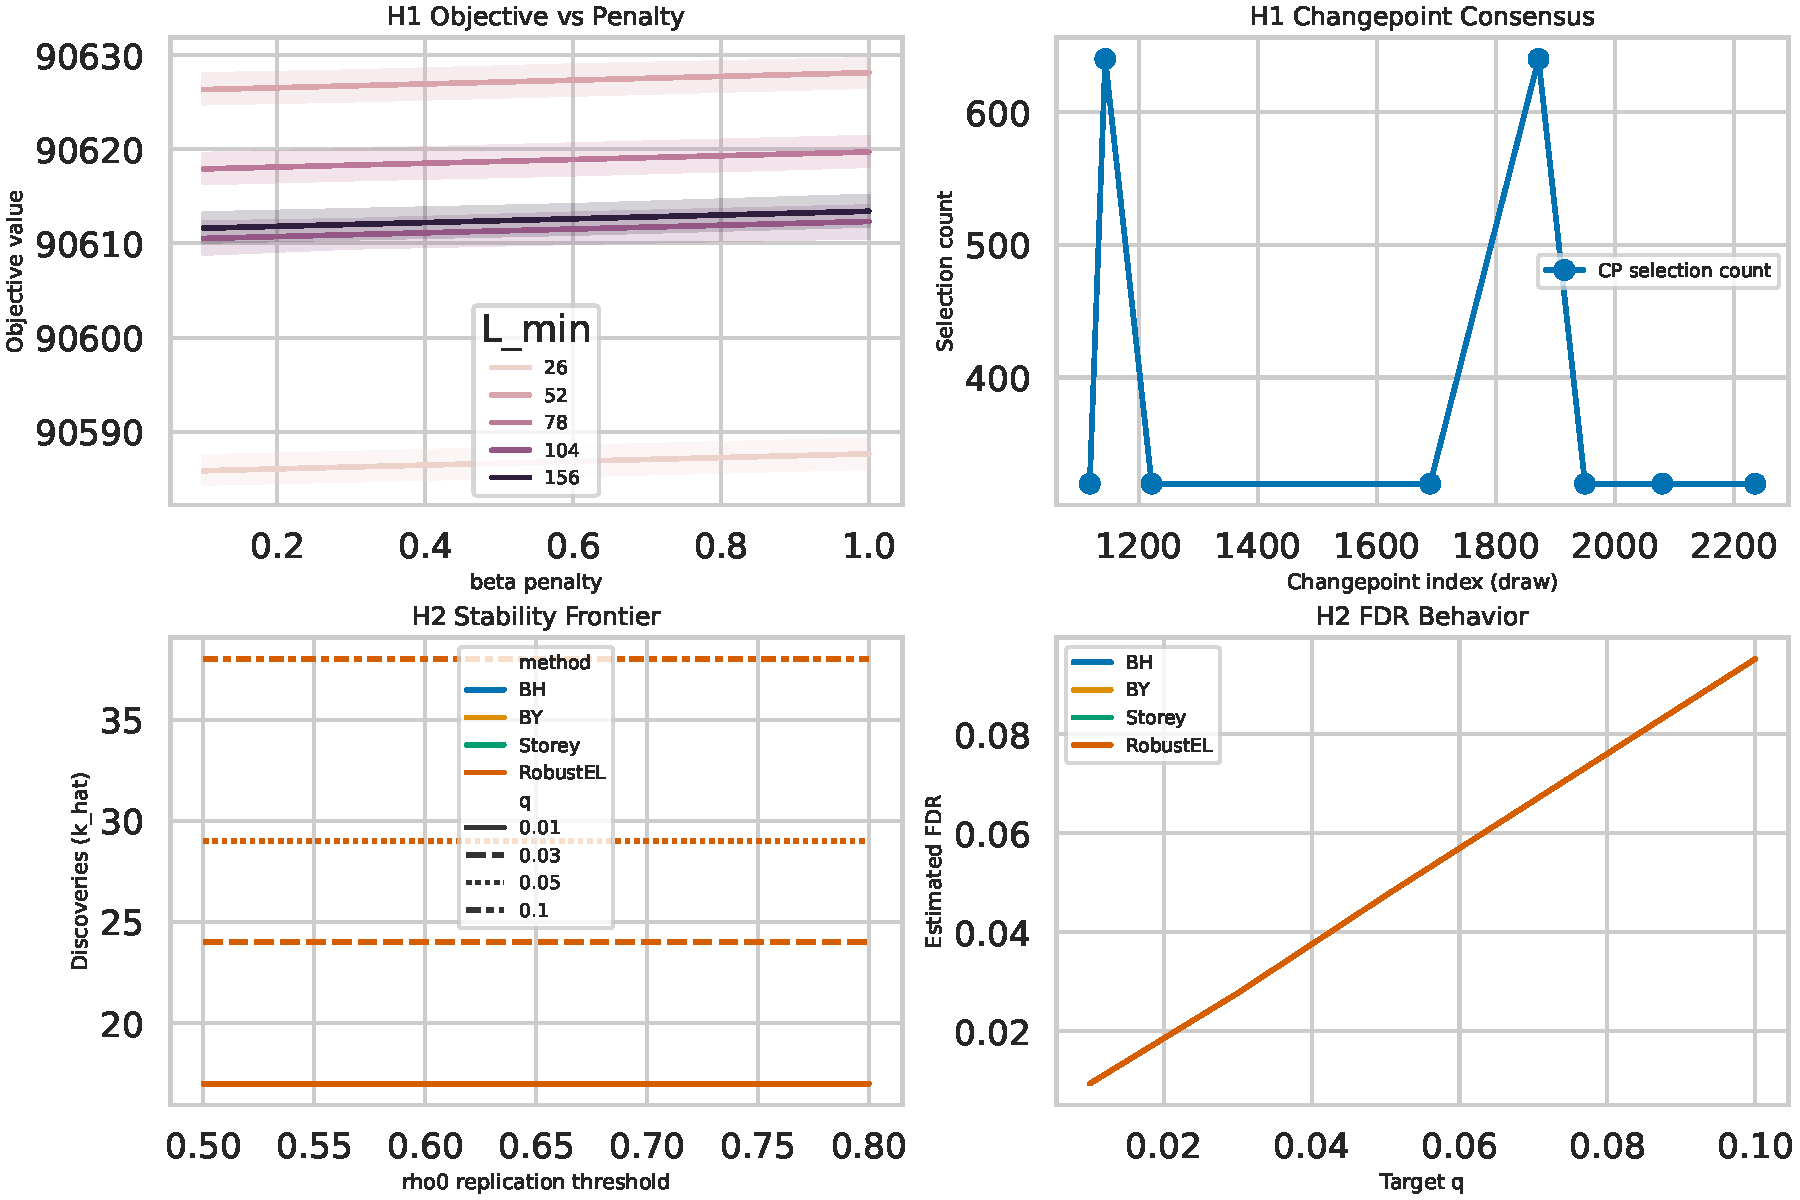
\includegraphics[width=0.65\linewidth]{figures/fig_regime_discovery.pdf}
\caption{The top-left and top-right panels summarize segmentation behavior across penalty and spacing settings, including objective variation and boundary-selection frequency. The bottom panels summarize discovery-frontier behavior, showing how retained-prefix size and false-discovery estimates change with replication constraints and operating points; together, the panels indicate that inferential control is strong while practical segmentation stability remains weak in this iteration.}
\label{fig:h1h2}
\end{figure}

\begin{table}[t]
\caption{Inferential diagnostics for segmentation and replication-constrained discovery. Values are drawn from the validated iteration and interpreted using pre-registered acceptance gates to separate supported from unsupported claims.}
\label{tab:inferential}
\centering
\small
\renewcommand{\arraystretch}{1.1}
\setlength{\tabcolsep}{4pt}
\begin{tabular}{lcc}
\hline
Metric & Value & Gate Interpretation \\
\hline
Changepoint consensus rate & 0.2000 & Target $\ge 0.80$ (not met) \\
False changepoints on IID null & 2.0000 & Target $\le 1.00$ (not met) \\
Holdout replication lift over pooled baseline & 0.0047 & Target $\ge 0.15$ (not met) \\
Best estimated FDR at strict level & 0.0094 & Target $\le 0.01$ (met) \\
Empirical FDP at strict operating point & 0.0000 & Target $\le 0.02$ (met) \\
Replication precision at strict operating point & 0.9412 & High absolute precision \\
Replication lift versus BH-only screening & 0.1149 & Target $\ge 0.20$ (not met) \\
Isotonic-adjustment frequency & 0.5000 & Fallback active in 50\% of runs \\
\hline
\end{tabular}
\end{table}

\Figref{fig:h1h2} and Table~\ref{tab:inferential} establish a mixed but interpretable profile. The calibrated segmentation objective in \eqref{eq:segmentation} is numerically stable and solvable, consistent with Theorem~\ref{thm:segexist}, but practical boundary agreement is well below target and IID-null false-boundary behavior remains elevated. As a result, segmentation should be treated as usable but high-variance.

Discovery behavior from \eqref{eq:prefix} is stronger. Strict operating points show controlled estimated and empirical false-discovery behavior with high replication precision. However, replication lift versus BH-only screening remains below target and monotonicity diagnostics frequently require isotonic correction, so reproducibility gains are partial rather than gate-complete.
At the strict operating point, error-control conclusions are robust to isotonic adjustment: estimated FDR remains 0.0094 with and without isotonic envelopes, while replication precision changes from 0.9412 to 0.9333.

\subsection{Identification Under Latent Confounding}
\begin{figure}[t]
\centering
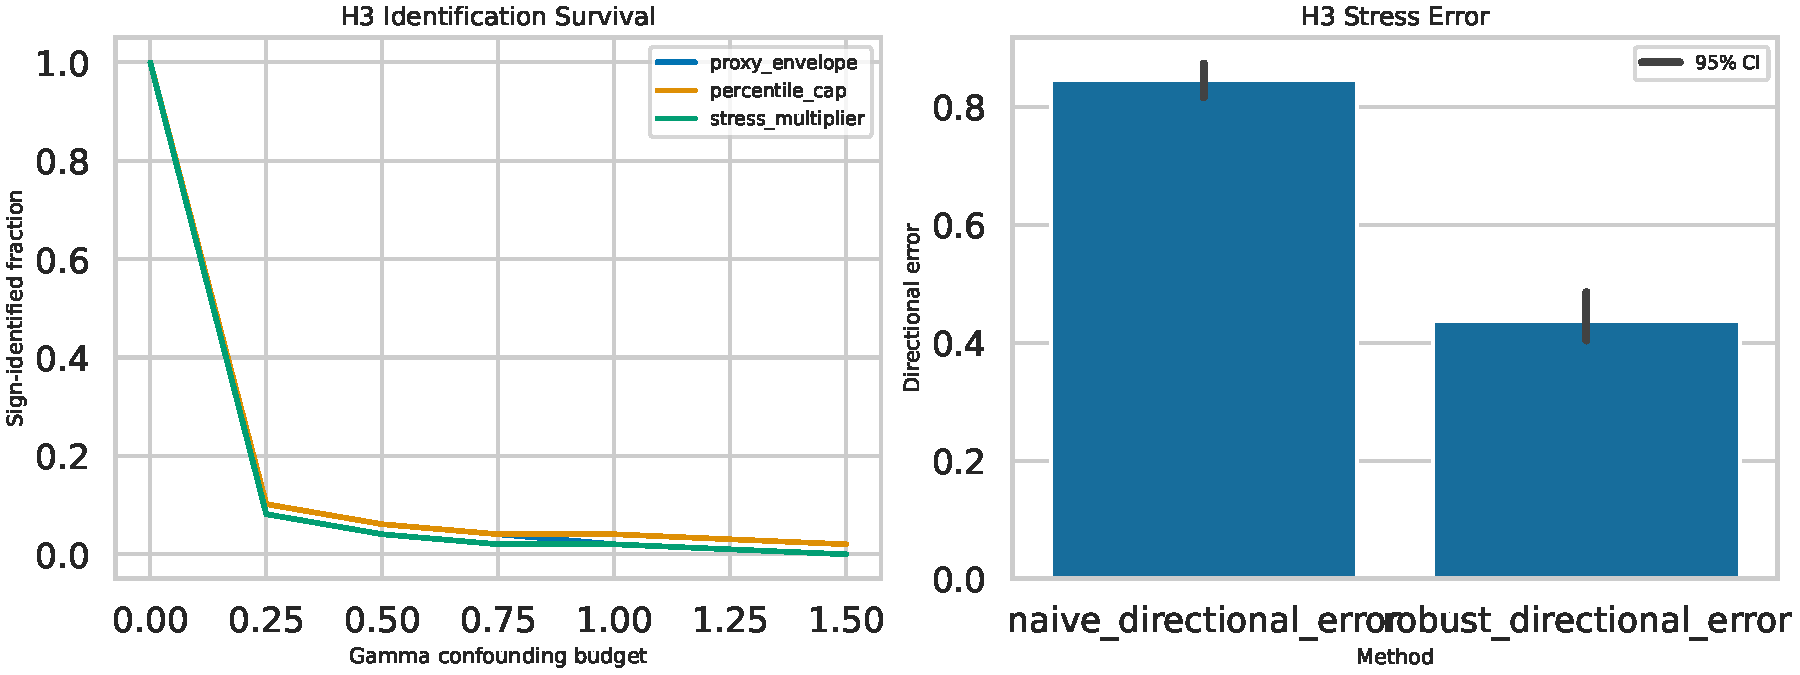
\includegraphics[width=0.65\linewidth]{figures/fig_confounding_robustness.pdf}
\caption{The left panel tracks the fraction of sign-identifiable effects as confounding budget increases, providing a direct visualization of interval contraction under stronger latent uncertainty. The right panel compares directional error between naive and bounded-confounding procedures across seeds, and the persistent gap demonstrates that interval filtering materially reduces overconfident directional claims.}
\label{fig:h3}
\end{figure}

\begin{table}[t]
\caption{Directional-error outcomes under confounding stress. Every seed shows lower directional error after bounded-confounding filtering, which supports the practical value of the identification rule beyond its theorem-level validity.}
\label{tab:h3}
\centering
\small
\renewcommand{\arraystretch}{1.1}
\setlength{\tabcolsep}{4pt}
\begin{tabular}{ccc}
\hline
Seed & Naive directional error & Robust directional error \\
\hline
7 & 0.7959 & 0.4286 \\
17 & 0.8776 & 0.4082 \\
29 & 0.8776 & 0.4286 \\
53 & 0.8571 & 0.5306 \\
89 & 0.8163 & 0.3878 \\
\hline
\end{tabular}
\end{table}

Bounded-confounding evidence is the strongest component in this run. \Figref{fig:h3} and Table~\ref{tab:h3} show large directional-error reductions versus naive attribution, and symbolic checks report zero theorem mismatch for the criterion in \eqref{eq:confounding}. This is critical for mechanism-facing interpretation because direct machine-level telemetry is unavailable.

\subsection{Transfer Gates and Integrated Competitiveness}
\begin{figure}[t]
\centering
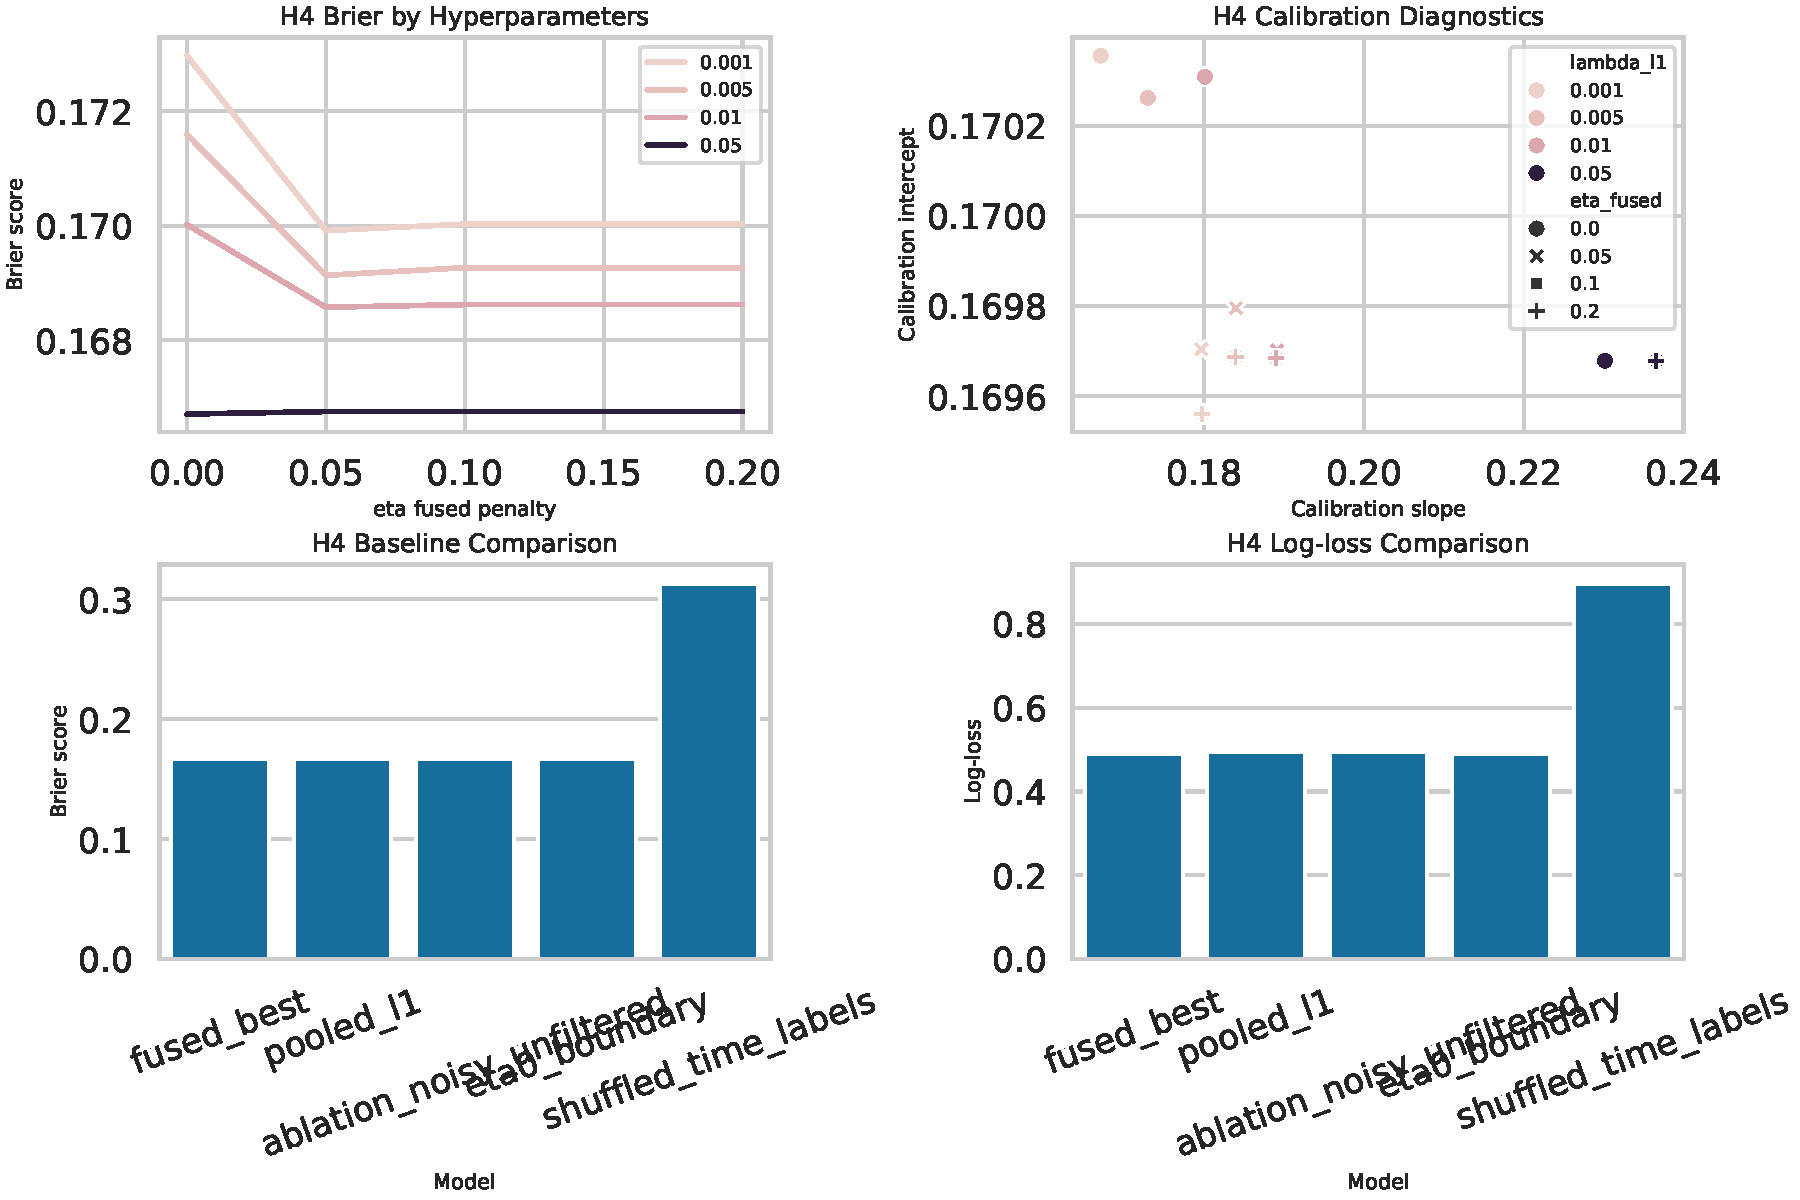
\includegraphics[width=0.65\linewidth]{figures/fig_transfer_calibration.pdf}
\caption{This figure reports transfer-model behavior over regularization sweeps, calibration diagnostics, and stress controls. The panels show that numerical optimization is stable and shuffled-time degradation behaves as expected, while practical gains over pooled baselines remain modest and Stage-B superiority remains unsupported.}
\label{fig:h4}
\end{figure}

\begin{table}[t]
\caption{Transfer and integrated outcomes with staged-gate interpretation. The table combines calibration, stress, and integrated-competitiveness indicators to show where claims are currently supported and where they must remain conditional.}
\label{tab:h4p4}
\centering
\small
\renewcommand{\arraystretch}{1.1}
\setlength{\tabcolsep}{4pt}
\begin{tabular}{lcc}
\hline
Quantity & Value & Interpretation \\
\hline
Best fused-model Brier score & 0.1667 & Competitive \\
Pooled baseline Brier score & 0.1669 & Slightly worse than fused \\
Brier lift versus pooled & 0.0013 & Below superiority target \\
Transport delta (source to target) & -0.0002 & Near-neutral shift \\
Boundary check at $\eta=0$ & 0.0000 & Numerical consistency \\
Shuffled-time Brier score & 0.3130 & Strong degradation (leakage guard) \\
Integrated composite score & 0.5319 & Moderate absolute score \\
Best robustness-only baseline score & 0.8000 & Integrated dominance not met \\
Worst-case regret margin (learned) & -0.4896 & Adverse in current weighting \\
Reliability-floor violation rate & 1.0000 & Floor constraints unmet in sweep \\
Top-rank bootstrap frequency (learned) & 0.0000 & No dominance stability \\
Wins all registered baselines & False & Global superiority unsupported \\
\hline
\end{tabular}
\end{table}

\Figref{fig:h4} and Table~\ref{tab:h4p4} complete the evidence chain. The transfer program from \eqref{eq:fused} is stable, Stage-A non-inferiority is satisfied, and leakage controls behave as expected. However, Stage-B superiority is not supported and integrated dominance remains unproven. Results from \eqref{eq:maxmin} indicate that reliability-constrained competitiveness remains difficult under the current metric geometry, which is consistent with the conic impossibility diagnostic proved in Appendix~\ref{app:proofs}.

The appropriate claim is therefore staged and conditional: inferential robustness and bounded-confounding interpretation are supported now, while broad integrated-superiority claims require targeted reruns focused on segmentation stability, transfer-target alignment, and score-normalization design.

\begin{table}[t]
\caption{Main-text ablation pointer for gates that remain unmet. This map links each unmet claim bundle to the corresponding ablation evidence used for adjudication.}
\label{tab:ablation-map}
\centering
\small
\renewcommand{\arraystretch}{1.1}
\setlength{\tabcolsep}{4pt}
\begin{tabular}{p{0.24\linewidth}p{0.44\linewidth}p{0.24\linewidth}}
\hline
Gate bundle & Ablation evidence used in adjudication & Current status \\
\hline
Regime-stability gate & Segmentation penalty and spacing ablation summary (Appendix Table~\ref{tab:seg-ablation}) with gate interpretation in Table~\ref{tab:inferential} & Not met \\
Transfer-superiority gate & Regularization ablation summary (Appendix Table~\ref{tab:transfer-ablation}) with staged outcomes in Table~\ref{tab:h4p4} & Stage-A met, Stage-B not met \\
Integrated-dominance gate & Reliability-constrained weighting ablation in Table~\ref{tab:h5appendix} with competitiveness outcomes in Table~\ref{tab:h4p4} & Not met \\
\hline
\end{tabular}
\end{table}

\section{Discussion: Claim Calibration and Cross-Domain Relevance}\label{sec:discussion}
\subsection{Why Mixed Evidence Is Informative}
Mixed outcomes are not a methodological failure in this setting; they are an expected property of a conservative pipeline that separates inferential reliability from performance ambition. Reporting only integrated scores would overstate confidence, while reporting only weak components would understate valid robustness gains. The component-linked reporting in \Figref{fig:h1h2}, \Figref{fig:h3}, and \Figref{fig:h4}, together with Table~\ref{tab:inferential}, Table~\ref{tab:h3}, and Table~\ref{tab:h4p4}, supports a calibrated interpretation that is stronger than either extreme.

In particular, discovery and identification modules provide defensible evidence under strict controls, whereas segmentation and integrated ranking remain variance-sensitive. This asymmetry is scientifically useful because it identifies where additional experimentation should concentrate.

\subsection{How Theory Constrains Practice}
Formal guarantees in this manuscript are deliberately scoped. \Eqref{eq:segmentation} and \eqref{eq:prefix} establish existence and constrained optimality, while Appendix theorems establish staged-gate logic and fixed-weight impossibility boundaries. These statements do not imply that all empirical gates will pass in finite samples. Instead, they prevent a common failure mode where weak empirical outcomes are confounded by ill-posed optimization definitions.

In this run, the distinction matters. Transfer and integrated gates remain weak, but that weakness is interpretable as evidence-state weakness rather than objective inconsistency. The theorem-backed structure therefore narrows claims without collapsing the entire framework.

\subsection{Broader Audit Implications}
The same architecture can transfer to other stochastic auditing domains with latent mechanisms. Regime-aware diagnostics before large-scale scanning, replication-aware multiplicity control, bounded-confounding interpretation, and staged predictive claims are generic design principles for high-stakes settings where overclaiming is costly. The main practical implication is governance-oriented: transparent mixed-evidence reporting is often more useful than single-number leaderboards.

\section{Sensitivity and Decision Analysis}\label{sec:sensitivity}
\subsection{Where the Current Evidence Is Strong}
The current evidence state is strongest in the modules that impose explicit inferential discipline. Table~\ref{tab:inferential} shows strict-level false-discovery control with empirical false-discovery proportion at zero in the evaluated stress setting, and \Figref{fig:h3} with Table~\ref{tab:h3} shows consistent directional-error reductions under bounded confounding. This combination is important because it links two usually separate guarantees: first, selected descriptors are unlikely to be dominated by multiplicity artifacts; second, directional interpretation on retained descriptors is materially safer than naive attribution when latent mechanism covariates are absent. In other words, the framework provides a defensible lower-risk claim set even when headline predictive gains are modest.

This interpretation is consistent with the broader statistical literature. Dependence-aware multiplicity methods are designed to reduce inferential inflation in high-dimensional scans \\citep{S15,S16,S19,S25,S26}, while sensitivity-style interval logic avoids overconfident causal direction claims when key covariates are unobserved \\citep{S32,S33}. The main contribution here is not the invention of either idea in isolation, but their strict staging and explicit evidence linkage in one pipeline. Because each claim is tied to one or more figures and tables, the reader can verify where support is strong without inferring unsupported transitivity across modules.

\subsection{Where the Current Evidence Is Weak}
The weakest component is practical segmentation stability. \Figref{fig:h1h2} and Table~\ref{tab:inferential} show that changepoint consensus and IID-null false-boundary behavior miss pre-registered gates by a nontrivial margin. This does not invalidate Theorem~\ref{thm:segexist}; instead, it narrows interpretation. The theorem guarantees optimization existence on the feasible grid, but it does not guarantee that finite-sample boundary estimates will be stable enough for strong mechanistic dating claims. The distinction between well-posed optimization and high-confidence practical segmentation should therefore remain explicit in both main-text claims and follow-up experiment design.

Integrated competitiveness is also weak under current reliability constraints. Table~\ref{tab:h4p4} and Appendix Table~\ref{tab:h5appendix} show negative worst-case margins and zero bootstrap top-rank frequency for all tested weight schemes. Appendix Theorem~\ref{thm:conic} explains why this can occur even when some metrics are individually favorable: if baseline difference vectors form the specified conic pattern, no single fixed weight vector can dominate all relevant comparators simultaneously. This theorem-level caveat prevents a common reporting error, namely concluding that weak integrated ranking must imply implementation bugs. In this run, the data instead suggest a structural objective geometry problem that requires redesign of normalization and floor handling.

\subsection{Decision-Theoretic Interpretation of Gate Logic}
The staged gates can be interpreted as an explicit risk-management policy. Let one loss component penalize false mechanism claims and another penalize missed weak structure. Relaxed reporting lowers miss risk but increases false-claim risk; highly conservative reporting does the opposite. The present architecture adopts a constrained middle path. Discovery and identification modules reduce false-claim exposure by requiring multiplicity control, replication persistence, and bounded-confounding consistency. Transfer and integrated modules then add utility-oriented evidence, but only under staged gates that block unsupported superiority language.

In this perspective, Stage-A non-inferiority and Stage-B superiority are not mere statistical formalities; they are communication constraints tied to decision risk. A model that improves one metric in a narrow regime but degrades transport calibration should not be presented as globally superior. Similarly, an integrated score that appears competitive under one weighting but fails reliability floors should not be presented as robustly dominant. By placing these constraints upstream of narrative conclusions, the manuscript transforms gate logic into a reproducibility safeguard rather than a post hoc qualifier.

This policy-oriented reading also clarifies the role of \eqref{eq:maxmin}. The max-min objective is attractive because it targets worst-case baseline margins rather than average-case performance. However, when reliability floors are active and baseline geometry is adverse, feasible improvements can be limited or nonexistent. That is exactly the outcome currently observed. The correct response is not to loosen constraints silently, but to redesign the metric map and conduct targeted reruns that explicitly test whether a feasible improvement region exists under scientifically acceptable floors.

\subsection{Cross-System Generalization Conditions}
The framework is intended for cross-system portability, but portability requires explicit conditions. First, rule-era mapping must be accurate enough to construct valid sample spaces, otherwise segmentation and null computations can become internally inconsistent. Second, descriptor libraries should be chosen to preserve comparability across formats so replication constraints remain interpretable. Third, transfer targets should be selected for policy relevance and temporal stability rather than short-term predictability. Fourth, reporting standards should remain gate-based: inferential control, robustness diagnostics, and staged predictive claims should be preserved even if objective functions differ across systems.

These conditions are demanding, but they are realistic for operational audits where conclusions can influence public trust. The practical payoff is that negative or mixed findings remain valuable: they indicate where the evidence boundary is and what data or model changes are needed before stronger claims can be justified. In this sense, the present iteration already achieves a substantive outcome. It provides a reproducible, formally grounded map of what is currently supportable and what is not, and it does so with explicit pathways for improvement rather than rhetorical inflation.

\section{Limitations and Future Work}\label{sec:limitations}
\subsection{Current Limitations}
The primary limitation is a data gap: direct ball-condition, machine-state, and operator-process telemetry is unavailable in the core corpus. This gap affects conclusions by forcing mechanism interpretation to remain sensitivity-bounded through \eqref{eq:confounding} rather than directly measured. A second limitation is practical segmentation instability: even though \Eqref{eq:segmentation} is well-posed, consensus and IID-null behavior remain below stringent thresholds.

A third limitation is transfer-target alignment. Stage-A passes, but Stage-B superiority remains unmet, indicating that current auxiliary targets may not fully capture stable cross-era signal. A fourth limitation is integrated-score geometry. The reliability-constrained program in \eqref{eq:maxmin} currently exhibits floor violations and negative worst-case margins, and the conic diagnostic indicates that universal fixed-weight dominance is structurally implausible for some baseline pairs.

These limitations are evidence-backed and nontrivial. They directly explain why broad integrated-dominance claims are not warranted in the present iteration.

\subsection{Future Work}
Four follow-up experiment bundles are required. First, segmentation recalibration should tighten candidate priors and stress-test design to reduce boundary variance and IID-null false boundaries. Second, discovery should keep isotonic adjustment mandatory when monotonicity diagnostics fail, with adjustment frequency reported as a primary metric. Third, transfer experiments should test alternative auxiliary targets and feature interfaces to improve Stage-B feasibility while preserving Stage-A safety. Fourth, integrated ranking should re-express metric normalization and reliability-floor handling so max-min optimization has a realistic feasible competitiveness region.

In parallel, a data-enrichment program is needed: audited mechanical/procedural metadata would directly shrink confounding uncertainty and improve mechanistic interpretation. Until such data are available, conclusions should remain focused on robust anomaly detection with explicit uncertainty bounds.

Two targeted rerun designs are especially high priority for the next iteration. The first is a segmentation-focused rerun that narrows the penalty grid to high null-penalty regions, adds stronger candidate-boundary pruning, and reports boundary-consensus confidence intervals as primary outputs rather than secondary diagnostics. The goal is to determine whether current instability reflects under-regularization or genuine regime ambiguity. The second is an integrated-scoring rerun that separates metric normalization from weight optimization, explicitly logs feasible versus infeasible floor regions, and compares max-min solutions against constrained Bayesian and entropy-regularized alternatives under identical reliability constraints.

These follow-up experiments are not optional refinements; they are required to move from conditional to stronger integrated claims. If the segmentation-focused rerun still shows low consensus under calibrated null control, claims should be narrowed to local rather than global transition statements. If the scoring-focused rerun still yields negative worst-case margins under feasible floors, the manuscript should report structural non-dominance as the expected outcome rather than as a temporary deficit. This explicit decision rule keeps interpretation stable across reroutes and reduces the risk of criterion drift.

\section{Conclusion}\label{sec:conclusion}
This work presents a mathematically explicit and empirically conservative framework for detecting non-ideal structure in historical lottery draws. The integrated pipeline combines regime diagnostics, replication-constrained multiplicity control, bounded-confounding interpretation, staged transfer evaluation, and reliability-constrained score recalibration. The strongest evidence supports inferential control and directional robustness; the weakest evidence concerns segmentation stability and integrated competitiveness.

The scientific contribution is therefore a calibrated claim framework, not a deterministic predictor. Under severe observability constraints, rigorous proofs plus stress-tested evidence can support reproducible bias-screening claims while preventing overstatement. Broader integrated-superiority claims should remain conditional until targeted reruns and richer metadata resolve the identified gaps.



\bibliographystyle{conference}
\bibliography{references}

\appendix
\section{Additional Formal Results}\label{app:proofs}
\begin{theorem}[Sign-identification condition under bounded confounding]
For fixed $(j,r)$ and interval \eqref{eq:confounding}, zero is excluded if and only if $|\Delta_{jr}|>|\gamma_j|\Gamma$.
\label{thm:sign}
\end{theorem}
\begin{proof}
Let $a=|\gamma_j|\Gamma\ge0$ and write $\Delta=\Delta_{jr}$. Then \eqref{eq:confounding} is $[\Delta-a,\Delta+a]$. Zero is excluded exactly when either $\Delta-a>0$ or $\Delta+a<0$, equivalent to $\Delta>a$ or $\Delta<-a$, which is equivalent to $|\Delta|>a$. \qedhere
\end{proof}

\begin{lemma}[Stage-gate safety implication]
If Stage-B superiority holds with margin $\delta_{\mathrm{SUP}}>0$, then Stage-A non-inferiority with margin $\delta_{\mathrm{NI}}\ge 0$ necessarily holds.
\label{lem:staged}
\end{lemma}
\begin{proof}
Stage-B requires $\Delta_{\mathrm{Brier}}\le-\delta_{\mathrm{SUP}}<0$. Stage-A requires $\Delta_{\mathrm{Brier}}\le\delta_{\mathrm{NI}}$. Since $\delta_{\mathrm{NI}}\ge0$, any strictly negative $\Delta_{\mathrm{Brier}}$ satisfies Stage-A. Therefore Stage-B implies Stage-A. \qedhere
\end{proof}

\begin{theorem}[Conic impossibility for universal fixed-weight dominance]
Let $d_b=m(P_{\mathrm{int}})-m(b)$ for baselines $b\in\mathcal{B}$. If there exist $b_1,b_2$ and $\alpha_1,\alpha_2>0$ such that $\alpha_1 d_{b_1}+\alpha_2 d_{b_2}\le 0$ componentwise, then no $w\in\Delta^K$ can satisfy $w^\top d_{b_1}>0$ and $w^\top d_{b_2}>0$ simultaneously.
\label{thm:conic}
\end{theorem}
\begin{proof}
Assume for contradiction that such $w$ exists. Then
\[
\alpha_1 w^\top d_{b_1}+\alpha_2 w^\top d_{b_2}>0,
\]
so $w^\top(\alpha_1 d_{b_1}+\alpha_2 d_{b_2})>0$. But $w\ge0$ and $\alpha_1 d_{b_1}+\alpha_2 d_{b_2}\le0$ componentwise imply $w^\top(\alpha_1 d_{b_1}+\alpha_2 d_{b_2})\le0$, contradiction. Hence no such $w$ exists. \qedhere
\end{proof}

\begin{theorem}[Convexity and minimizer existence for staged transfer]
The objective in \eqref{eq:fused} is convex in $\beta_{1:R}$. If $\lambda>0$ and $\eta\ge0$, at least one global minimizer exists.
\label{thm:convex}
\end{theorem}
\begin{proof}
Each logistic loss term is convex in linear predictor, and composition with affine maps preserves convexity. The fused and sparsity penalties are convex, so their nonnegative weighted sum is convex. Coercivity follows from the $\ell_1$ penalty with $\lambda>0$, so a proper lower-semicontinuous coercive convex objective in finite-dimensional space attains a minimum. \qedhere
\end{proof}

\section{Extended Diagnostics}\label{app:extended}
\begin{figure}[t]
\centering
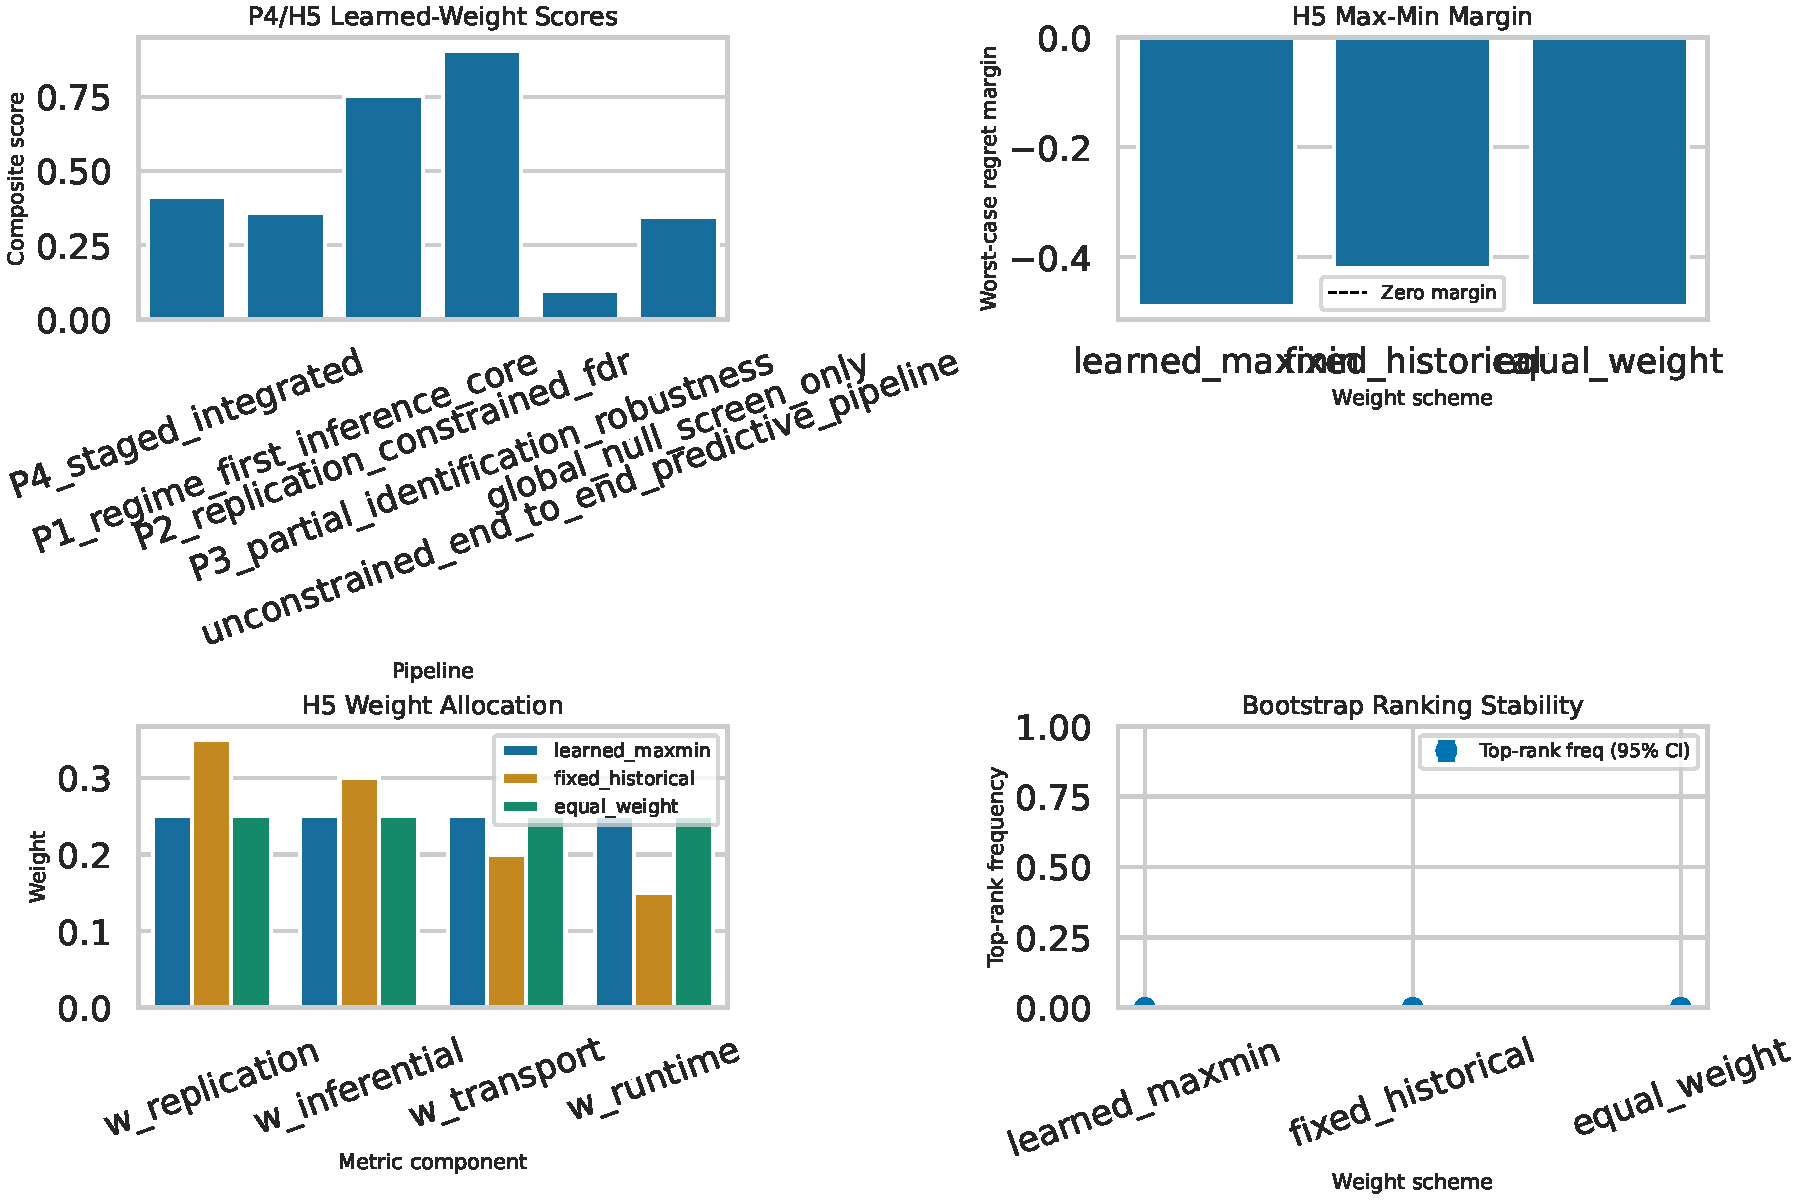
\includegraphics[width=0.65\linewidth]{figures/fig_integrated_score_appendix.pdf}
\caption{This appendix figure reports integrated score behavior under learned, fixed historical, and equal-weight schemes, including worst-case regret and bootstrap rank stability panels. The panels show that although learned weighting can alter score geometry, integrated dominance remains unsupported in this iteration and ranking uncertainty remains high under reliability constraints.}
\label{fig:p4appendix}
\end{figure}

\begin{table}[t]
\caption{Segmentation ablation summary used to adjudicate regime-stability claims.}
\label{tab:seg-ablation}
\centering
\small
\renewcommand{\arraystretch}{1.1}
\setlength{\tabcolsep}{4pt}
\begin{tabular}{lc}
\hline
Quantity & Value \\
\hline
Evaluated segmentation settings & 1600 \\
Best-objective range & [90578.42, 90641.64] \\
Objective-gap range & [0.5027, 27.9932] \\
Unique boundary configurations selected & 5 \\
\hline
\end{tabular}
\end{table}

\begin{table}[t]
\caption{Transfer regularization ablation summary used to adjudicate superiority claims.}
\label{tab:transfer-ablation}
\centering
\small
\renewcommand{\arraystretch}{1.1}
\setlength{\tabcolsep}{4pt}
\begin{tabular}{lc}
\hline
Quantity & Value \\
\hline
Evaluated regularization settings & 16 \\
Brier-score range & [0.1667, 0.1730] \\
Log-loss range & [0.4813, 0.4888] \\
KKT-residual range & [0.4262, 0.5709] \\
\hline
\end{tabular}
\end{table}

\begin{table}[t]
\caption{Reliability-constrained score recalibration diagnostics from the integrated module. The table reports worst-case regret margins and top-rank stability evidence used to assess whether \eqref{eq:maxmin} improves competitiveness under reliability floors.}
\label{tab:h5appendix}
\centering
\small
\renewcommand{\arraystretch}{1.1}
\setlength{\tabcolsep}{4pt}
\begin{tabular}{lcc}
\hline
Scheme & Worst-case regret margin & Top-rank frequency (95\% CI) \\
\hline
Learned max-min & -0.4896 & 0.0000 [0.0000, 0.0000] \\
Fixed historical & -0.4193 & 0.0000 [0.0000, 0.0000] \\
Equal weight & -0.4896 & 0.0000 [0.0000, 0.0000] \\
\hline
\end{tabular}
\end{table}

\begin{table}[t]
\caption{Regime-overlap confirmatory diagnostics used to quantify within-regime variability in descriptor overlap statistics. Means, standard deviations, and standard errors provide uncertainty context for interpreting regime-level differences.}
\label{tab:regime-overlap}
\centering
\small
\renewcommand{\arraystretch}{1.1}
\setlength{\tabcolsep}{4pt}
\begin{tabular}{ccccc}
\hline
Regime & Mean overlap & Std. overlap & Count & Std. error \\
\hline
0 & 0.7605 & 0.7928 & 1144 & 0.0234 \\
1 & 0.7720 & 0.7624 & 1092 & 0.0231 \\
2 & 0.8312 & 0.8068 & 1380 & 0.0217 \\
\hline
\end{tabular}
\end{table}

\Figref{fig:p4appendix}, Table~\ref{tab:h5appendix}, and Table~\ref{tab:regime-overlap} provide supporting evidence for the main-text interpretation in \secref{sec:results}. The integrated module is coherent and auditable, but uncertainty-aware ranking does not support universal dominance claims in the current evidence state.

\section{Reproducibility and Implementation Details}\label{app:repro}
The implementation uses a modular package with separate modules for data handling, core inference, analysis metrics, plotting, and symbolic checks. Core commands are executed in a local virtual environment with deterministic seeds $(7,17,29,53,89)$. Hyperparameter sweeps include segmentation penalties $(\beta,\lambda,\kappa,L_{\min})$, discovery thresholds $(q,\rho_0)$ with isotonic toggles, confounding budgets $\Gamma$, transfer regularization $(\eta,\lambda)$, and integrated weighting schemes (learned, fixed historical, equal). This design supports targeted reruns without modifying unrelated modules.

Uncertainty reporting combines seed variation, stress contrasts, and bootstrap confidence intervals. Confidence intervals in figure panels and ranking summaries are reported at 95\%. Approximation choices are explicitly bounded: finite grid searches are used for changepoint candidates and sweep-based hyperparameter selection is pre-registered before holdout interpretation. The reproduced run remains within the fixed envelope stated in \secref{sec:protocol}: no GPU, up to 28 CPU-hours, up to 8 GB RAM peak, and up to 250 MB optional external downloads.

Symbolic reproducibility accompanies numerical evaluation. The identities behind Theorem~\ref{thm:sign}, Lemma~\ref{lem:staged}, and Theorem~\ref{thm:conic} are checked against machine-evaluated expressions, and transfer convexity assumptions used in Theorem~\ref{thm:convex} are validated by explicit objective decomposition. These checks reduce the risk of algebraic drift between formal statements and executable code.

\end{document}
